
\chapter{理论实验}

\section{实验设定说明}
\subsection{实验目标}
检验本文提出的误差估计方法的有效性,关键是要看“真实”的震源机制是否包含在反演的震源机制估计值的误差范围内。而对权重优化方案的评估,则是以联合加权相比于独立加权,其反演结果的稳定性和可靠性是否被更全面地考虑为评判标准。

检验误差估计方法有效性时,需要事先知道“真实”的震源机制,用于评判反演结果是否真实可靠。为此,设计了一个已知震源机制的理论实验,本实验假定震源的相关参数为$M_w$震级6.5,震源深度17km,其震源机制为走向250$\degree$,倾角40$\degree$,滑动角82$\degree$。该参数设置仿照了之后应用实例的相关参数,便于与之后的类似结果进行相互印证。

为了考察联合定权相对单独定权的优化性,需要评价结果的可靠性和稳定性,以比较三种加权方案的可靠性和稳定性的差异。可靠性的评价理论上以结果的期望与真值的一致性为准,在实际计算中则以反演所给的最优震源机制与真值间的偏差大小为依据。而稳定性则是讨论数据噪声对反演结果的影响,通常影响越大,观测数据与理论预测值的匹配程度也会越低,在本文的反演方法中体现为拟合度Fit越低。

\subsection{参数设定}
由于计算的是远震事件波形,选择了ak135全球结构速度模型\citep{Kennett1995},它是横向均匀的一维速度模型。理论地震图和相应格林函数库的计算均使用波数积分法完成,计算了震中距为4500km的8个台站的理论波形。为了确保数据分布满足约束要求,给反演提供足够优良的数据结构,得以将关注点集中在其它需要对照的条件上,选定的8个台站方位角分别设置为0°、45°、90°、135°、180°、225°、270°、315°。为方便表述,将这8个方位角从小到大的台站依次称为STA1、STA2、STA3、STA4、STA5、STA6、STA7、STA8,其分布如\reffig{fig3_01}所示。各台站理论计算的原始无噪波形如\reffig{fig3_02}所示。
\begin{figure}
\centering
  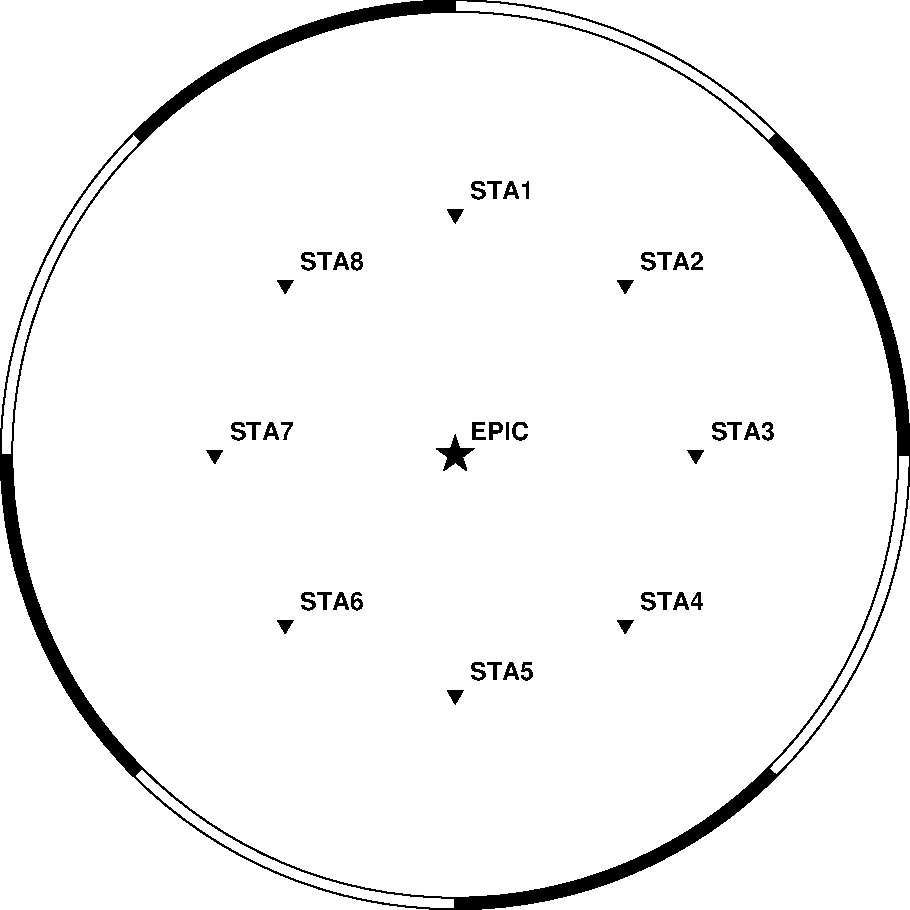
\includegraphics[scale=0.5,angle=0]{fig3_01.pdf}
  \caption{理论实验的台站分布,其中五角星表示震中,倒三角表示台站}
  \label{fig3_01}
\end{figure}
\begin{figure}
\centering
  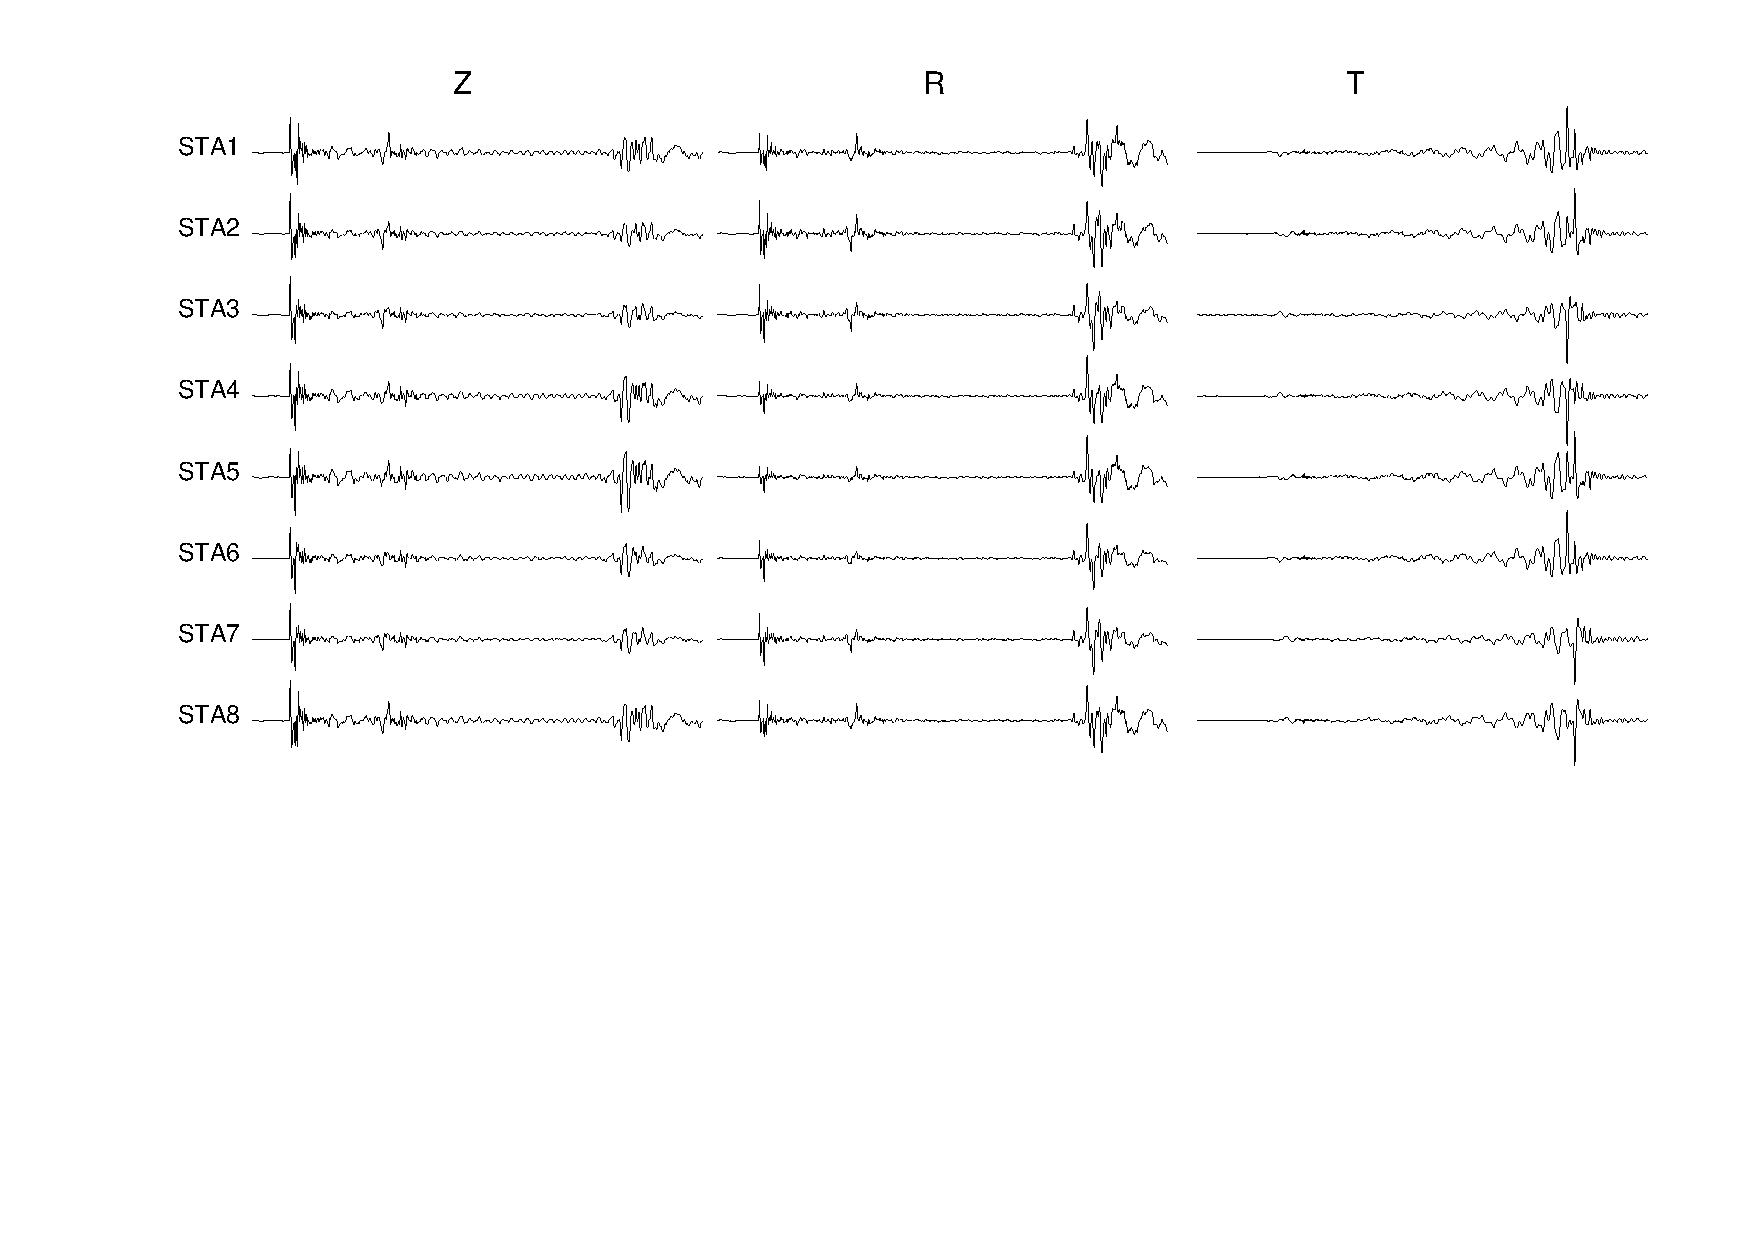
\includegraphics[scale=0.5,angle=-90]{fig3_02.pdf}
  \caption{理论实验中通过波数积分法计算的各台站理论波形}
  \label{fig3_02}
\end{figure}

\subsection{实验条件检验}
为了保证实验条件设定合理,满足原始数据对反演的约束力度,便于后续实验的结果分析。我们首先检验了利用理论计算的无噪数据反演的情况,在该情况下,信噪比已经最大化,加权以及滤波等处理并不会有影响。基于Fit互相关拟合标准,利用格点搜索反演算法对该理论波形进行反演。发现反演结果与设定的震源参数完全一致,结果很可靠,说明对于该反演,所提供的各台站数据有很好的分布结构。反演结果对应的拟合度Fit值为1(最高值,代表完全拟合),由于数据无噪声,结果的误差范围为0,十分稳定。高信噪比数据对应稳定的反演结果,证明了拟合度Fit的高低确实能表征结果稳定性。同时,拟合度为1也表明了在反演过程中计算机内数值计算的舍入、截断误差影响可忽略不计。

\section{权重优化检验}

\subsection{实验条件}
本文提出的权重优化方案是基于前人单独考虑振幅比加权或信噪比加权的方案,进行了联合定权。为了实际检验联合加权是否如理论分析一般,有效综合了两种单独加权的益处,对反演结果有优化作用,设置了三组对照实验组用于检验。对照组对比加权的影响,因此除加权外三组的其它条件均相同。基于CPS的Fit拟合函数进行格点搜索反演,采用前文章节的理论事件设定和台站波形数据。第一组对照组在反演时采用W1单独加权,第二组对照组则改为W2单独加权,第三组为了试验本文加权方案效果采用W1和W2联合之后的WT加权方案。

为了体现信噪比权重W1的作用,对理论波形添加了噪声。加噪时参考了实际数据中的噪声平均强度为$10^{-6}m$量级,并稍微提高了噪声振幅值,以增强三组对照组反演结果由W1加权影响导致的差异明显性。将中误差为$5\cdot10^{-6}m$的高斯白噪声作为原始噪声加入理论波形中。W2加权的作用在于合理调节不同振幅的波形数据在反演中的影响力,由于所设定的8个台站均处于同一震中距,震中距引起的衰减作用相同。为了使数据有明显振幅差异,反演时将P波震相和S波震相分别从波形中截取出来,并用P波和S波联合反演,以尽可能体现振幅比调节权重W2在反演中的作用。

\subsection{结果分析}

三组对照组反演得到的结果如\reftab{tab3_01}所示,可以发现即使在数据结构较好的情况下,使用完全一样的反演数据,以及同一反演程序,三组反演的结果还是有可见差异的。经过不同加权反演后,虽然结果均离真值偏差不大,但明显可以看到,W1加权反演组拟合度最高,因为它尽可能抑制噪声影响,降低高噪声数据权重,以追求整体数据的最大拟合度,其震源机制也与真值较接近,但震源深度却与真实深度偏差了1km。而W2加权对照组虽然没有经过信噪比加权,拟合度在三组中最差,可震源深度却没有明显偏差,不过震源机制比W1略差。对于WT联合加权反演组,由于同时考虑了数据信噪比以及数据不同振幅权重,其拟合度情况不致于太低,而且综合来看震源深度和震源机制更接近真值(虽然差异不大,但考虑到毕竟是完全一样的反演数据)。
\begin{table}[ht]
\centering
\caption{三种加权方案得到的解}
\label{tab3_01}
    \begin{tabular}{c c c c c c c}
    \hline
     & 走向/$\degree$ & 倾角/$\degree$ & 滑动角/$\degree$ & 深度/km & 拟合度(Fit) & 震级($M_w$)\\
    \hline
    真值	& 250 & 40 & 82 & 17 & 1	& 6.50\\
    W1		& 252 & 40 & 82 & 18 & 0.91 & 6.52\\
    W2		& 245 & 39 & 78 & 17 & 0.75 & 6.47\\
    WT		& 250 & 40 & 81 & 17 & 0.84 & 6.50\\
    \hline
    \end{tabular}
\end{table}

以下分别从数据源差异,拟合度意义和加权的直接影响针对反演结果进行分析。

反演数据源主要包括P波和S波数据,在纯剪切位错源情况下,所激发的S波震相的振幅要明显高于P波振幅。但这两震相数据所加的噪声强度是相同的,因而两种数据中,S波的信噪比相对较高。

另一方面,与P震相接近的远震pP及sP震相对震源深度具有较好的约束作用。因为pP或sP的传播路径和P波的传播路径非常相似,如\reffig{fig3_03}所示仅在震源处有不可忽略差异。这种特性能很好地消除它们在远震传播情况下,走时差受中间长距离传播过程中所受介质模型误差的影响。在合理的近似下,它们的到时差仅来源于震源处初始传播路径的差异\citep{Stein2003}。以pP波和P波的差异为例,如\reffig{fig3_04}所示,假设该小区域速度均匀无变化,则两者的到时差可以近似为\refeq{eq3_01},其中$\alpha$为该区域P波的速度。同理可推得sP震相与P震相的到时差为\refeq{eq3_02},可以看到到时差${\delta}t_{pP}$和${\delta}t_{sP}$只依赖于震源深度、入射角和震源区域速度,和台站方位角、地震波传播路径中速度以及震源机制均无关,所以反演结果可能出现震源机制好,但震源深度差的情况(W1加权反演组)。在本文理论实验的速度模型、震中距和P时窗截取长度条件下,pP震相和sP震相已经包含在截取的P波时窗中,这意味着该实验中P波数据相较于S波对震源深度的约束更强。 
\begin{equation}
\label{eq3_01}
{\delta}t_{pP}=(2hcosi)/\alpha
\end{equation}
\begin{equation}
\label{eq3_02}
{\delta}t_{sP}=(h/\alpha)(cosi+(3-sin^2i)^{1/2})
\end{equation}

\begin{figure}
\centering
  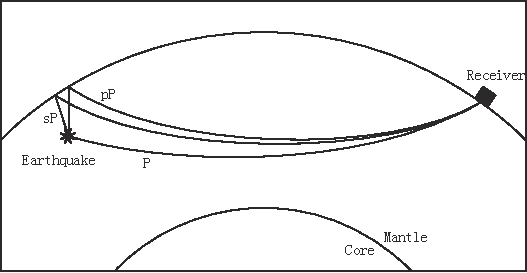
\includegraphics[scale=1.1]{fig3_03.pdf}
  \caption{远震情况下P,sP,pP震相的传播路径\citep{Stein2003}}
  \label{fig3_03}
\end{figure}
\begin{figure}
\centering
  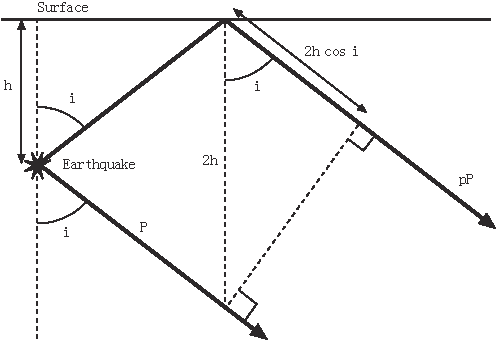
\includegraphics[scale=1.1]{fig3_04.pdf}
  \caption{远震情况下P,pP震相的走时差分析\citep{Stein2003}}
  \label{fig3_04}
\end{figure}

在格点搜索过程中通过各格点计算的拟合度高低来直接选定最优解。考虑到波形中所加的噪声是随机白噪声,具有高度随机性,决定了它基本不可能被理论波形完全拟合。所以噪声在干扰反演结果的同时,也伴随着数据拟合度降低,反演受随机噪声的影响越大,其拟合度通常相应会越低。因此拟合度Fit暗示了噪声对结果的干扰程度,代表了结果稳定性优劣。

W1信噪比加权反演组对高信噪比的S波赋予了较大权重,加之S波本身的高振幅更使得反演中S波数据对反演结果占主导作用,最终导致其结果拟合度在三组对照组中最高。但正因为P波的贡献被减弱,因而P波的深度约束能力没能很好体现,导致该组反演的震源深度在三组对照组中有唯一可见偏差(超过了1km格点搜索精度)。对于W2加权对照组,由于进行了振幅调节加权,振幅大的S波权重相对削弱,而P波的作用加强,使低振幅的P波在反演中能有同等影响力,所以深度得到了较好约束。然而在放大P波信号权重的同时也放大了P波中噪声的权重,考虑到P波信噪比较低,在P波中占比较大的噪声也在反演中对结果起到了更严重的干扰作用,理所应当的拟合度会降低,较低的拟合度象征着结果较差的稳定性。最后,联合信噪比和振幅调节的WT加权反演组,一方面通过振幅调节权重W2对具有振幅差异的不同波形合理分配了权重,使得具有不同振幅的P波和S波信息均在反演中有相对平等的贡献,另一方面同时施加的W1权重在一定程度上压制了高噪声对震源反演的干扰。最终反演结果的拟合度处于W1单独加权对照组和W2单独加权对照组之间,反演结果具有可接受的稳定性,并且更多的有用信息使得对震源机制和震源深度的整体约束作用更强,结果更为可靠。

\subsection{结论}
以上分析说明,信噪比权重W1针对数据信噪比进行优化,有效地压制了噪声在反演中的影响,保证了预测数据和观测数据间较高的吻合程度,提高了结果的稳定性。振幅调节加权W2则从数据结构着手,通过对不同振幅的波形数据合理分配权重,间接增加了数据总体的信息,对待求参数约束更全面,使反演结果更为真实、可靠。本文结合了W1和W2的联合加权方案WT,同时吸收了两种单独加权的优点,反演时综合考虑了数据信噪比和数据结构两方面,在一定程度上优化了反演,得到的解从整体看更稳定、可靠,WT联合加权确实有优化效果。

\section{误差评定方法检验}

\subsection{理论实验误差评价过程}
虽然前面章节已经完整描述了将误差评价方法应用于实际案例的流程,并将其分为了三大步。但在理论实验中应用上述方法还有一点点不同,因为实际应用时已经从观测台站获取了天然地震激发的地震波DATA0,在理论事件中需要人工合成DATA0。
因此,我们需要在第一步之前加上一步——合成恰当的原始“观测波形”。由于原始观测波形的信噪比对反演结果的误差有很大影响,为了使理论实验有参考意义,需要谨慎、合理地添加噪声。
本文采用高斯白噪声给理论波形加噪,以模拟最原始的“观测”数据。随机噪声的期望必定为零,分布函数中只有一个标准差参数需要设定,它代表了噪声的强度。

由于获得误差评价的过程较繁琐,此处将之前各大步骤中的细分小步统一进行描述,以清晰地描述在理论实验中反演并获得误差评价的详细过程。

利用本文的误差估计方法,对理论实验中震源机制进行反演并估计误差的完整步骤如下:1.生成原始观测数据DATA0,该步是理论实验特有的,设置原始噪声强度(即高斯分布标准差),并生成该强度下随机高斯白噪声,将白噪声加至理论波形中,视为台站处接收到的“观测波形”DATA0;2.首先估计原始噪声,用参数估计方法对DATA0中每道数据波形分别估计其噪声的强度,估计时选取P波到达前的空白震相期波形作为该道波形的噪声数据样本,并将其视为符合高斯分布的序列,从而可利用参数估计得到该噪声分布的标准差;3.而后模拟等价噪声,利用上一步得到的DATA0中各道波形噪声的标准差分别生成与原波形时窗长度相等的高斯白噪声序列;4.生成模拟带噪数据,将上步生成的高斯白噪声与DATA0中各道波形对应相加,便得到了第一套模拟带噪数据DATA1;5.生成多套模拟数据,重复步骤2、3、4,每重复一次可得到一套新的模拟带噪数据DATAi,假设一共重复N次,便得到DATA1,DATA2...,DATAN,总共N套模拟数据;6.重复反演得到解集,对原始观测数据和模拟数据中的每套数据DATAi(i=0,1,2..N),采用同样的数据处理方式和权重方案,基于CPS进行独立反演,总共重复反演N+1次,得到的对应的震源机制解Mi(i=0,1,2,...N);7.统计解集得到误差信息,利用统计方法对Mi(i=0,1,2...N)样本进行估算得到协方差及相关系数信息。至此便在用“观测”数据反演得到最优震源机制M0的同时得到了震源机制参数的协方差等误差信息。

在理论实验的每次独立反演过程中,均采用同样的数据处理方式,并用震相中的P波与S波(SV,SH)进行联合反演。为了尽可能模拟真实情况,数据进行了时窗截取,噪声滤波等处理。P波数据截取了相对P波到时(-10s,30s)的时窗,并进行(0.01Hz,0.1Hz)带通滤波;SH波滤波频率为(0.05Hz,0.1Hz),时窗选为相对其震相到时(-20s,40s)的范围;SV波的波形与其它震相交叠延续,时窗设定较长,为相对到时(-30s,150s)范围。需要注意,在实际应用中,由于SPL(shear coupled wave,远震SV的后续波)存在,导致SV波形受地壳上地幔结构影响较大,一般不能用于震源参数反演\citep{Aki1980},但在理论实验中没有结构误差影响,因此可以使用。在格点搜索过程中为保证效率和精度分步进行,第一步全空间快速搜索,步长为10$\degree$,大步长确保搜索效率,第二步在上一步搜索的最优点附近进行局部精搜索,步长为1$\degree$,小步长确保了搜索精度。由于误差评价方法需要重复搜索,若将深度也加入搜索范围会导致巨量的计算时间,因此只在计算M0时加入了震源深度搜索,之后为误差评定进行的搜索仅针对震源机制的走向、倾角和滑动角三个参数,而深度设定为第一次计算M0搜索到的最优深度。

\subsection{检验目标}
由于波形拟合反演公式复杂,而且反演数据量大,推演得到数据噪声到震源机制误差的传播矩阵非常困难。因此在该理论模拟实验中,给定数据误差的情况下,依然无法直接得到震源机制的误差期望用于检验。

在对本文误差评价方法有效性的理论检验实验中,我们将设置了两个检验目标。一是检验误差是否具体其应有的作用——确保理论真值在反演结果的误差范围内,这是对误差评价最基本也最重要的要求;二是检验结果的误差大小是否满足其应有的特性——与原始噪声强度有正相关关系,根据误差传播规律,最终的震源机制误差为误差传播矩阵与原始数据噪声的乘积。

\subsection{对照组设定}
为检验该两目标,设置多组对照组进行反演,每组对照组仅有的数据原始噪声强度大小不同,其余条件均一致。每一组实验的反演结果均可与设定的理论事件震源参数真值直接比较,而检验真值是否在结果误差范围内,误差评价是否准确。而通过进行各组间误差大小的差异对比,可以分析误差与数据噪声的相互关系是否合理,以检验误差的性质。

对照组共分为4组,各组噪声均为高斯白噪声,考虑到波形的振幅强度基本为$10^{-5}$m量级,而实际噪声强度则在$10^{-6}$m左右,将噪声标准差大小分别设置为低噪声组$1.0\cdot10^{-6}$m,中噪声组$2.5\cdot10^{-6}$m,高噪声组$5.0\cdot10^{-6}$m,超高噪声组$1.0\cdot10^{-5}$m,并将误差评价方法中重复反演总次数N+1定为100。

\subsection{结果及讨论}
通过向四组对照组的理论波形加入不同强度的高斯白噪声,相应生成了四组信噪比不同的“观测波形”DATA0,分别独立用于各组的反演及误差评定中。经搜索反演和本文误差估计,得到了各组震源机制最优值,相应的误差协方差和震源机制间各参数的相关性。其中低强度噪声组、中等强度噪声组、高强度噪声组和超高强度噪声组的误差协方差和相关性分别如\reftab{tab3_02}、\reftab{tab3_03}、\reftab{tab3_04}和\reftab{tab3_05}所示。
\begin{table}[ht]
\centering
\caption{低强度噪声组误差协方差和相关性}
\label{tab3_02}
    \begin{tabular}{c c c c}
    \hline
    协方差 & 走向/$\degree$ & 倾角/$\degree$ & 滑动角/$\degree$ \\
    \hline
	走向/$\degree$ 		&1.06	 	&-0.04		&0.53\\
	倾角/$\degree$		&-0.04		&0.13		&0.02\\
	滑动角/$\degree$	&0.53		&0.02		&0.71\\
    \hline
    \end{tabular}
    \begin{tabular}{c c c c}
    \hline
    相关系数 & 走向/$\degree$ & 倾角/$\degree$ & 滑动角/$\degree$ \\
    \hline
	走向/$\degree$ 		&1 			&-0.10		&0.61\\
	倾角/$\degree$		&-0.10		&1			&0.06\\
	滑动角/$\degree$	&0.61		&0.06		&1\\
    \hline
    \end{tabular}
\end{table}

\begin{table}[ht]
\centering
\caption{中强度噪声组误差协方差和相关性}
\label{tab3_03}
    \begin{tabular}{c c c c}
    \hline
    协方差 & 走向/$\degree$ & 倾角/$\degree$ & 滑动角/$\degree$ \\
    \hline
	走向/$\degree$ 		&5.78		&-0.30		&3.77\\
	倾角/$\degree$		&-0.30		&0.57		&0.36\\
	滑动角/$\degree$	&3.77		&0.36		&4.99\\
    \hline
    \end{tabular}
    \begin{tabular}{c c c c}
    \hline
    相关系数 & 走向/$\degree$ & 倾角/$\degree$ & 滑动角/$\degree$ \\
    \hline
	走向/$\degree$ 		&1 			&-0.16		&0.70\\
	倾角/$\degree$		&-0.16		&1			&0.21\\
	滑动角/$\degree$	&0.70		&0.21		&1\\
    \hline
    \end{tabular}
\end{table}

\begin{table}[ht]
\centering
\caption{高强度噪声组误差协方差和相关性}
\label{tab3_04}
    \begin{tabular}{c c c c}
    \hline
    协方差 & 走向/$\degree$ & 倾角/$\degree$ & 滑动角/$\degree$ \\
    \hline
	走向/$\degree$ 		&34.85	 	&-5.30		&25.80\\
	倾角/$\degree$		&-5.30		&3.27		&-4.70\\
	滑动角/$\degree$	&25.80		&-4.70		&32.76\\
    \hline
    \end{tabular}
    \begin{tabular}{c c c c}
    \hline
    相关系数 & 走向/$\degree$ & 倾角/$\degree$ & 滑动角/$\degree$ \\
    \hline
	走向/$\degree$ 		&1 			&-0.50		&0.76\\
	倾角/$\degree$		&-0.50		&1			&-0.45\\
	滑动角/$\degree$	&0.76		&-0.45		&1\\
    \hline
    \end{tabular}
\end{table}

\begin{table}[ht]
\centering
\caption{超高强度噪声组误差协方差和相关性}
\label{tab3_05}
    \begin{tabular}{c c c c}
    \hline
    协方差 & 走向/$\degree$ & 倾角/$\degree$ & 滑动角/$\degree$ \\
    \hline
	走向/$\degree$ 		&101.05 	&-1.05		&101.85\\
	倾角/$\degree$		&-1.05		&20.11		&5.61\\
	滑动角/$\degree$	&101.85		&5.61		&141.26\\
    \hline
    \end{tabular}
    \begin{tabular}{c c c c}
    \hline
    相关系数 & 走向/$\degree$ & 倾角/$\degree$ & 滑动角/$\degree$ \\
    \hline
	走向/$\degree$ 		&1 			&-0.02		&0.85\\
	倾角/$\degree$		&-0.02		&1			&0.11\\
	滑动角/$\degree$	&0.85		&0.11		&1\\
    \hline
    \end{tabular}
\end{table}
假设震源机制各参数的可能误差范围为其误差分布标准差大小的3倍,进一步考虑到在格点搜索反演时的搜索精度为1$\degree$,可得到4组对照组反演的最终震源机制和其可能误差范围如\reftab{tab3_06}所示。
\begin{table}[ht]
\centering
\caption{加不同强度原始噪声得到的解及误差范围}
\label{tab3_06}
    \begin{tabular}{c c c c c}
    \hline
    加噪强度 & 走向/$\degree$ & 倾角/$\degree$ & 滑动角/$\degree$ &最高拟合度 \\
    \hline
    无噪声		& 250 & 40 & 82  & 1\\
    低噪声		& 250$\pm$3 & 40$\pm$3 & 82$\pm$3 & 0.99 \\
    中等噪声	& 250$\pm$8 & 40$\pm$3 & 83$\pm$7 & 0.94 \\
    高噪声		& 246$\pm$18 & 40$\pm$6 & 78$\pm$17 & 0.87 \\
    超高噪声	& 245$\pm$30 & 42$\pm$14 & 84$\pm$36 & 0.65 \\
    \hline
    \end{tabular}
\end{table}

从\reftab{tab3_06}可以发现在四组对照组中震源机制的真值均包含在其估计的误差范围内,即使在超高噪声情况下,最优震源机制相对真值出现了较明显偏差,其偏差仍然远小于误差范围,说明估计的误差是可信的。原始数据由于包含一定强度随机噪声,会使结果出现一定程度内的随机偏差,本文误差估计的本质在于准确估计了噪声强度,并通过多次模拟该强度噪声数据并重复反演,统计出了该强度噪声影响下对结果影响的程度,从而通过附加该程序的误差范围使有偏差的解得以“纠正”回真值。

此外,从\reftab{tab3_06}还可以看出随着噪声强度的增强,各组震源机制对应参数的误差范围也相应增大,因为噪声越大,对结果的随机干扰越强,误差范围要相应变大以满足将随机干扰包含在其内部。数据的拟合度Fit有效地反映了噪声的干扰程度,也即结果的稳定性。通过\reftab{tab3_06}可以发现,各对照组的噪声越大,误差范围越大,拟合度越低,而结果的稳定性也越差。此外,在同一参照组中,走向、倾角和滑动角的误差大小不同,稳定性也不同。总的看来对该震源机制反演,倾角的稳定性最好,对噪声最不敏感。

进一步对误差进行定量对比,根据\refeq{eq2_19},可以发现若我们将所有观测数据噪声${\triangle}d$的标准差均同时增大$n$倍,通过线性性质推导,其反演结果误差协方差矩阵的各项元素,在理论上其期望应同时增大$n^2$倍。这种线性传导性质将得到两个结论,第一个是由于误差协方差增大$n^2$倍,则震源机制三个参数误差的标准差在理论上其期望也应增为原来的$n$倍。第二个是误差协方差各无素同时增大同一倍数,并不会影响其元素比值计算得到的相关系数矩阵,相关系数矩阵的期望不变。

接下来对以上两个关于误差信息定量变化的性质进行验证。在对照组的噪声设定中,每个台站及每个分量的噪声强度均设置为相同。从低噪声组到高噪声组,噪声的标准差分别为$1.0\cdot10^{-6}$m,$2.5\cdot10^{-6}$m,$5.0\cdot10^{-6}$m,$1.0\cdot10^{-5}$m,后组噪声强度分别恰好增强为之前组的2倍。从\reftab{tab3_06}可以发现,除了中等强度噪声组的倾角误差不是低强度噪声组的2倍,对其它参数,稍强噪声组的误差范围(3倍标准差)均近似为稍弱噪声组的误差范围两倍。之所以只满足近似性相等,一方面是2倍的定量关系是针对期望而言,样本统计不可能正好等于期望,另一方面\refeq{eq2_19}是针对线性问题推导,本文震源机制波形反演是非线性的,在解附近误差的线性分析也是利用了局部近似原理,依然会有少量偏差。综上,在概率统计意义上,各对照组对应震源机制参数的误差大小比值恰好等于其原始数据噪声强度的比值。
对比各对照组震源参数的相关系数矩阵,可以发现各参数间的相关系数在不同噪声组中基本一致(差异不大,可以用统计偏差进行解释),不随噪声强度变化而明显改变,符合对于相关系数矩阵性质的推论。

此外,综合考虑\reftab{tab3_02}、\reftab{tab3_03}、\reftab{tab3_04}和\reftab{tab3_05}中三个参数间相关系数矩阵,从统计意义上发现在此反演中走向和滑动角有较强正相关性,走向和倾角则只有微弱的负相关性,而倾角和滑动角间具有较弱的正相关性。两个参数相关系数的符号暗示了受到噪声影响时,两参数偏差的变化趋势关系。相关系数为正,表示两个参数与真值的偏差可能同号——同时偏大或同时偏小,而相关系数的绝对值则表明了这种可能性大小。相关系数矩阵预测了震源机制各参数受扰动时的变化模式,是反演结果误差的相关性信息,表明各参数偏差在概率上并非是杂乱无章的。

\subsection{结论}
从反演结果可以看出,在不同噪声强度的对照组中,所给出的最终结果的误差范围内均包含真值——走向250°,倾角40°,滑动角82°,验证了本实验的第一个目标——误差范围的准确性。本次不同噪声强度的对照实验表明本文误差估计方法可靠,其有效地反映了不同数据随机噪声对反演结果造成的误差。从随机性角度分析,一次反演的结果可能在误差范围内取任意不可预料值。各组实验均有不同程度的误差,表明即使用信噪比较高的,数据结构分布很好的优质数据作为输入数据,反演时得到的结果仍然可能与真值有一定偏差。因此,在格点搜索反演震源机制时,即使数据随机噪声强度较低,其影响也超过了搜索精度,仍然不可忽略,表明了误差分析的必要性。

另一方面,随着原始数据噪声逐渐增强,其反演结果的误差范围也会伴随着增长,以保证真值在误差范围内。误差大小与数据噪声强度基本保持正比例关系,符合关于误差性质检验的第二个目标以及理论推论。且误差相关系数矩阵基本不受噪声强度影响,与理由预测相符合。相关系数预示了震源机制各参数的误差间关系,是误差的附加信息。

随着反演结果的误差逐渐变大,稳定性变差,其数据拟合度也相应降低,其参考性和科学意义也随之降低。如在本实验中,噪声强度和有效波形振幅相当的超高噪声情况下,震源机制误差已经高于30°,基本超出了某些需要精确结果以参考的应用的可接受范围,科学价值较低。该结果体现了原始数据对于反演结果的重要性,原始数据质量决定了最终结果的优劣。
由于原始数据质量从根本上决定了最终结果好坏,及包含的科学意义,在实际工作中应该筛选优质观测数据,及时剔除不可靠或劣质数据。为了模拟真实观测数据的信噪比,后续理论反演中将噪声强度设置为中等强度,即$2.5\cdot10^{-6}$m。

\section{误差评定反演次数测试}
\subsection{实验目的}
在本文的误差评价方法中,主要利用随机统计原理,需要进行多次重复反演。从统计学理论可知,为了满足样本对全体估计的可靠度,要求样本具有良好随机性,且样本容量不能过小。

为了保证统计样本的随机性,在本文的误差评价方法中,每一次重复反演时,均对数据的每一道波形中每一个采样点的噪声进行了随机生成。并且生成时按照独立同高斯分布函数进行,保证了统计要求的随机性。而每一道波形包含了大量的采样点,数据全体有不同台站不同分量的多道波形,因此总采样点数很大,大量采样点噪声的随机生成足以满足噪声统计时,原始噪声的随机性和样本容量大小要求。

此外,在本文提出的误差评价方法中还有一个关于模拟数据的反演次数参数N,N需要人为设定。N代表了对噪声随机影响估计的总次数,也直接决定了最后分析评估震源机制误差协方差矩阵和相关系数信息所用的样本容量大小。从理论上讲,N应该尽量设置大,以保证足够多的样本采样量。但是随着N的增长,由重复反演带来的计算量也在同步线性增长。为了减少重复反演中的计算负担,已经将对模拟数据反演时的深度搜索去掉,但总计算量仍然不容小看。事实上,由于样本容量无法达到无穷大,估计总是会出现偏差。虽然容量越大偏差越小,但这种变化并不是线性关系,在样本容量较小时,容量的增大对偏差的减小很明显,容量达到一定大小后,样本数量的增加对估计偏差的影响已经不那么显著。所以从计算效率和准确性两方面综合考虑,需要在方法应用中选择一个合理的N值。

\subsection{实验方法}
为了确保重复反演次数设置合理,使误差统计方法有效的同时计算速度不至于太慢,需要确定较合理的N值。在此设置了一个对照实验,各对照组除N值外,其它条件均相同,用以对比寻找出比较适宜的N值。总共设置了4组对照组,按从小到大的顺序,分别将重复反演总次数N+1设置为10,50,100,200。

由于使用相同的数据,理论上误差也应一致,各参照组所估计的是同一目标误差。但是如前所述,随着N增大,估计量的更准确的概率也越来越大,误差估计值逐渐趋于稳定。所以我们要选择的最优参照组,需要同时保证误差范围有效,即包含真值,且在该样本容量之后,N值的增加对误差的影响相对较小。

本实验是理论事件的震源机制反演和误差估计,详细的反演过程与前文对误差估计方法有效性的估计是一样的,具体操作可参考之前章节。台站数据、滤波和加权均按之前所述方案,并且同样使用了P波和S波联合反演。唯一要注意的是在本实验反演过程中,参考之前噪声强度对比实验和实际数据噪声,将理论生成的原始观测数据噪声强度设置为中等强度——$2.5\cdot10^{-6}$m。

\subsection{结果及讨论}
为了方便对比不同参照组的反演结果,将各对组结果统一列入\reftab{tab3_07}中。以下分析不同N对反演的影响,找寻合适的N参数。
\begin{table}[ht]
\centering
\caption{不同重复反演总次数对应的震源机制及误差标准差}
\label{tab3_07}
    \begin{tabular}{c c c c c c c c}
    \hline
    重复次数 & 走向/$\degree$ & 标准差/$\degree$ & 倾角/$\degree$ & 标准差/$\degree$ & 滑动角/$\degree$ & 标准差/$\degree$\\
    \hline
    真值		& 250 & 0.00 & 40 & 0.00 & 82 & 0.00 \\
    10			& 250 & 1.85 & 40 & 0.87 & 83 & 1.74 \\
    50			& 250 & 2.20 & 40 & 0.68 & 83 & 1.99 \\
    100		& 250 & 2.39 & 40 & 0.71 & 83 & 2.00 \\
    200		& 250 & 2.46 & 40 & 0.87 & 83 & 2.04 \\
    \hline
    \end{tabular}
\end{table}

因为各参考组使用相同的原始观测数据,且所加噪声为中等强度,为节省数据生成的计算时间,直接采用了之前不同噪声强度对比实验中生成的中等强度噪声观测数据。由于原始数据相同,反演加权方法也一致,故各组得到的最优反演结果也相同,均为(走向250$\degree$,倾角40$\degree$,滑动角83$\degree$)。估计值与真值非常接近,若以误差标准差的3倍作为误差范围,在各参照组的误差范围内居严格包含震源机制真值。说明在几组试验组中,误差都是有效的。

反演结果及统计误差均有一定随机性,对各参照组估计的误差进行对比,找寻误差关于N相对较稳定的点。发现总反演次数N+1=10的时候,其结果与总反演次数为50的参照组相比,走向标准差差异高达-0.35,倾角标准差差异为0.19,滑动角标准差差异为-0.25。这是因为样本容量10较小,估计的稳定性较差,估计结果出现较大偏差的概率也大,当容量增到50时,样本容量由为10的欠缺情况下增加,其结果的改善会较为明显。继续分析总重复反演次数从50次增长到100次的结果差异,其走向、倾角和滑动角的标准差差异分别为0.19、0.03和0.01,相比于上一次的显著差异,变化开始平缓了。而总重复反演次数继续增加到200次,相比于100次的结果,其标准差差异对应于走向、倾角和滑动角分别为0.07、0.16和0.04,依旧较为平缓。这说明对该实验中随机性较好的统计样本,当样本容量大小在50-200的范围,容量大小对于随机统计而言已经相对充足,故容量大小的改变对估计结果的影响并不大。但在容量比较大的情况下,样本容量扩大一倍带来的计算时间会相应增加很长。因此在估计量变化较为平缓的情况下,不应以大幅降低计算效率为代价,为了结果少量的可能优化而继续增加样本容量,在折衷考虑下,认为各参照组中最优的选择方案是重复反演总次数为100的参照组。

\subsection{结论}
各参照组反演结果的误差范围内均包含理论真值,表明各反演对照组的结果均较可靠。在大量采样点噪声随机生成的高度随机性保证下,当重复反演总次数达到100左右,统计的误差结果对参数N不是很敏感,表明此时样本容量较充足。随着N的继续增加,误差估计的变化越来越微小,但重复反演带来的计算压力却仍增长显著。应用中可根据实际情况和硬件能力考虑N的取值,本文根据对比实验结果认为误差评价方法的重复反演总次数以100次为宜,也即将N设定为99。
